\PassOptionsToPackage{unicode=true}{hyperref} % options for packages loaded elsewhere
\PassOptionsToPackage{hyphens}{url}
%
\documentclass[]{article}
\usepackage[]{mathpazo}
\usepackage{setspace}
\setstretch{1.25}
\usepackage{amssymb,amsmath}
\usepackage{ifxetex,ifluatex}
\usepackage{fixltx2e} % provides \textsubscript
\ifnum 0\ifxetex 1\fi\ifluatex 1\fi=0 % if pdftex
  \usepackage[T1]{fontenc}
  \usepackage[utf8]{inputenc}
  \usepackage{textcomp} % provides euro and other symbols
\else % if luatex or xelatex
  \usepackage{unicode-math}
  \defaultfontfeatures{Ligatures=TeX,Scale=MatchLowercase}
\fi
% use upquote if available, for straight quotes in verbatim environments
\IfFileExists{upquote.sty}{\usepackage{upquote}}{}
% use microtype if available
\IfFileExists{microtype.sty}{%
\usepackage[]{microtype}
\UseMicrotypeSet[protrusion]{basicmath} % disable protrusion for tt fonts
}{}
\IfFileExists{parskip.sty}{%
\usepackage{parskip}
}{% else
\setlength{\parindent}{0pt}
\setlength{\parskip}{6pt plus 2pt minus 1pt}
}
\usepackage{hyperref}
\hypersetup{
            pdftitle={Improving Deconvolution Methods in Biology through Open Innovation Competitions: an Application to the Connectivity Map},
            pdfauthor={Author 1; Author 2; \ldots{}},
            pdfkeywords={biology, open innoation competitions, crowdsourcing, deconvolution, gene expressions, cell lines},
            pdfborder={0 0 0},
            breaklinks=true}
\urlstyle{same}  % don't use monospace font for urls
\usepackage[margin=1.25in]{geometry}
\usepackage{longtable,booktabs}
% Fix footnotes in tables (requires footnote package)
\IfFileExists{footnote.sty}{\usepackage{footnote}\makesavenoteenv{longtable}}{}
\usepackage{graphicx,grffile}
\makeatletter
\def\maxwidth{\ifdim\Gin@nat@width>\linewidth\linewidth\else\Gin@nat@width\fi}
\def\maxheight{\ifdim\Gin@nat@height>\textheight\textheight\else\Gin@nat@height\fi}
\makeatother
% Scale images if necessary, so that they will not overflow the page
% margins by default, and it is still possible to overwrite the defaults
% using explicit options in \includegraphics[width, height, ...]{}
\setkeys{Gin}{width=\maxwidth,height=\maxheight,keepaspectratio}
\setlength{\emergencystretch}{3em}  % prevent overfull lines
\providecommand{\tightlist}{%
  \setlength{\itemsep}{0pt}\setlength{\parskip}{0pt}}
\setcounter{secnumdepth}{5}
% Redefines (sub)paragraphs to behave more like sections
\ifx\paragraph\undefined\else
\let\oldparagraph\paragraph
\renewcommand{\paragraph}[1]{\oldparagraph{#1}\mbox{}}
\fi
\ifx\subparagraph\undefined\else
\let\oldsubparagraph\subparagraph
\renewcommand{\subparagraph}[1]{\oldsubparagraph{#1}\mbox{}}
\fi

% set default figure placement to htbp
\makeatletter
\def\fps@figure{htbp}
\makeatother

\usepackage{bbm}
\newcommand\hl{}
\newcommand\Fig{Fig. XXXX}

% Custom AB
\usepackage{booktabs}
\usepackage{longtable}
\usepackage{array}
\usepackage{multirow}
\usepackage[table]{xcolor}
\usepackage{wrapfig}
\usepackage{float}
\usepackage{colortbl}
\usepackage{pdflscape}
\usepackage{tabu}
\usepackage{threeparttable}
\usepackage{threeparttablex}
\usepackage[normalem]{ulem}
\usepackage{makecell}
\renewcommand*{\arraystretch}{1.2}


\title{Improving Deconvolution Methods in Biology through Open Innovation
Competitions: an Application to the Connectivity Map}
\author{Author 1 \and Author 2 \and \ldots{}}
\date{Last updated: Aug 22, 2019}

\begin{document}
\maketitle
\begin{abstract}
Report results fo open innovation competition aimed at solving a
gene-related deconvolution problem.


\smallskip\noindent 
Keywords: biology; open innoation competitions; crowdsourcing; deconvolution; gene expressions; cell lines.
\end{abstract}

{
\setcounter{tocdepth}{2}
\newpage
\tableofcontents
\newpage
}
TODOS:

\begin{itemize}
\tightlist
\item
  Intro AB
\item
  Methdos TN
\item
  Figure Scatter runtime vs accuracy for top10 TN
\item
  Add data
\end{itemize}

Here's a figure \ref{pic1}.

\hypertarget{introduction}{%
\section{Introduction}\label{introduction}}

Many recent examples have shown significant benefits for drug discovery
from the systematic analysis of large repositories of gene-expression
profiles {[}Refs{]}. However, traditional gene-expression
high-throughput profiling technologies that are based multianalyte
methods, such as Luminex profiling technology, are limited by the type
and number of available analytes {[}Refs{]}. Therefore, the cost of big
data generation in biology remains prohibitive.

The Connectivity Map (CMap) group at the Broad Institute has developed a
novel approach that matches pairs of genes to the same Luminex beads to
double the count of profiled genes per bead, thus lowering costs. A
central component of this approach is to quantify gene-type frequency of
beads, and then statistically deconvolve and compare gene type-specific
average expression profiles for pairs of mixed gene samples.

This type of deconvolution problems are ubiquitous and have a long
history in biology {[}refs{]}. For example, one common deconvolution is
used to identify cell type--specific gene expression differences in
complex tissues {[}Shen-orr et al., 2010{]}; or the discovery of the
target proteins of small molecules {[}Jung, 2015{]}.

Common approaches are parametric (mixture models) and non-parametric.
CMap's approach was K-nearest neighbors (KNN) approach. {[}Explain
briefly.{]} This works well but has several problems as well. {[}List
problems.{]} Including time. The trade-off between accuracy and
computation time is currently unknown.

Alternative methods are well known, such as Gaussian etc. But it would
have required substantial resources to experiment with these alternative
approaches (more than what already done) and to adapt new to our data.
Moreover, impossible an exhaustive search for all available approaches
to try; and the combination of these different approaches.

Instead, we used an open innovation competition as a research tool to
engage a variety of computer scientist, software developers and
bioinformatics in the problem. This allowed a simultaneous exploration
of competing approaches tailored to our problem, at no cost.

\hypertarget{methods}{%
\section{Methods}\label{methods}}

In biomedical research, our focus here, deconvolution problems are
common in multianalyte assay methods. These methods are widely used to
do X, Y and Z. In general terms, multianalyte assay methods are based on
microspheres with different fluorescence decay times. This feature can
be used to do X, Y, and Z. {[}EXPLAIN BRIEFLY CMap PROBLEM{]}. One
problem with existing approaches is that they {[}\ldots{}. {]}

To identify accurate methods we launched an open challenge that allowed
a rapid exploration of different approaches. Key ingredients of there
challenges are: training and testing dataset benchmark solution to
improve

\hypertarget{statistical-deconvolution-of-gene-specific-expression-profiles.}{%
\subsection{Statistical deconvolution of gene-specific expression
profiles.}\label{statistical-deconvolution-of-gene-specific-expression-profiles.}}

Assume fluorescent-intensity values \(X_{ij}\) for beads
\(i=1,2,\dots, n\) and analytes \(j=1,2,\dots, J\), and gene-specific
proportions \(w_{ik}\) for beads \(i=1,2,\dots, n\) and genes
\(k=1,2,\dots, K\). Our model of analyte fluourescent intensity is: \[
  X_{ij} = \sum_{k=1}^{K} w_{ik} h_{kj} + e_{ij}. 
\] where \(h_{ik}\) is the gene-expression value for genes
\(k=1,2,\dots, K\) and analytes \(j=1,2,\dots, J\).

For the UNI detection method, the gene-specific proportions are such
that each analyte has only one gene. Hence, \(w^{\text{uni}}_{ik} = 1\)
when \(j = k\), and it is zero otherwise. This implies that each sample
can detect at most \(J\) different genes under the UNI method.

For the DUO detection method, the gene-specific proportions are such
that each analyte is paired with two genes in 1:2 ratio. Hence, pick an
element \(g\in G^2\) from the set \(G^2\) of all non-overlapping subsets
of size two of the gene set \(G\). For each pair of genes in \(g\)
associated with an analyte \(j\), we have:
\(w^{\text{duo}}_{i1} = 2/3\), \(w_{i2}=1/3\) and is zero otherwise.

\hypertarget{data-generation}{%
\subsection{Data generation}\label{data-generation}}

To generate data for this contest, we profiled six 384-well perturbagen
plates, each containing mutually exclusive sets of compound and shRNA
treatments. Multiple treatment types were used to ensure avoid
potentially over-fitting to any one. The compound and shRNA perturbagen
plates were arbitrarily grouped into pairs, and to avoid any potential
`information leakage' each pair was profiled in a different cell line.
The resulting lysates were amplified by ligation mediated amplification
(LMA, Subramanian 2017). The amplicon was then split and detected in
both one-gene-per-bead (UNI) and two-genes-per-bead (DUO) detection
modes. The three pairs of data were arbitrarily assigned to training,
testing, and holdout categories, where in each case the UNI data served
as the ground truth.

The data so generated were then split into three subsets called:
training, provisional testing, and system testing. Training and
provisional-testing data were made available for all the contestants to
develop and validate their solutions, while system-testing data were
secured to evaluate competitors' last submissions, which was used to
award the prizes, and to avoid overfitting as well.

\begin{longtable}[]{@{}ll@{}}
\caption{Data generated}\tabularnewline
\toprule
Category & Type\tabularnewline
\midrule
\endfirsthead
\toprule
Category & Type\tabularnewline
\midrule
\endhead
training & Compounds\tabularnewline
provisional testing & Compounds\tabularnewline
system testing & Compounds\tabularnewline
training & shRNA\tabularnewline
provisional testing & shRNA\tabularnewline
system testing & shRNA\tabularnewline
\bottomrule
\end{longtable}

\hypertarget{to-read}{%
\subsection{To read}\label{to-read}}

\begin{itemize}
\tightlist
\item
  \href{https://pubs.rsc.org/en/content/getauthorversionpdf/c4mb00677a}{Compound
  signature detection on LINCS L1000 big data} used a fuzzy c-means
  Gaussian Mixture Model (GMM) to process raw L1000 data, showing better
  performance compared to KNN. This method is described below:
\end{itemize}

\begin{quote}
To deconvolute such overlapped peaks, we assumed that the fluorophore
intensities of each analyte type (corresponding to a specific mRNA type)
had a Gaussian distribution. The distribution of the mixture of analytes
GeneH(i) and GeneL(i) corresponding to the expression levels of GeneH
and GeneL, respectively, should be subject to a bimodal Gaussian
distribution, with the proportion of 1.25 to 0.75. We initialized the
estimations of the two Gaussian distributions using buzzy c-means
clustering {[}11{]} and estimated the GMM parameters using the
Nelder-Mead method {[}12{]}. Thus, the overlapped peaks were
deconvoluted as the two estimated Gaussian peaks and the expression
levels of the two genes sharing the same analyte were extracted.
Mathematical details are included in the Supplementary Methods (the GMM
model).
\end{quote}

\begin{itemize}
\item
  \href{https://ieeexplore.ieee.org/abstract/document/4044778}{Deconvolution
  of linear systems by constrained regression and its relationship to
  the Wiener theory}
\item
  \href{https://www.nature.com/articles/nmeth.2929}{Efficient
  Bayesian-based multiview deconvolution}
\item
  \href{https://www.nature.com/articles/nbt1414}{A Bayesian
  deconvolution strategy for immunoprecipitation-based DNA methylome
  analysis}
\item
  \href{https://www.nature.com/articles/nmeth.1830}{Gene expression
  deconvolution in linear space}
\item
  \href{https://www.nature.com/articles/nmeth.1439}{Cell type--specific
  gene expression differences in complex tissues}
\end{itemize}

\hypertarget{results}{%
\section{Results}\label{results}}

\hypertarget{participation}{%
\paragraph{Participation}\label{participation}}

The contest attracted xxx participants, who made xxx code submissions (a
median of xxx per person).

Fig. 1. Participation stats (Submission counts)

\hypertarget{overall-accuracy-and-speed.}{%
\paragraph{Overall accuracy and
speed.}\label{overall-accuracy-and-speed.}}

Fig. 2. (A) Leaderboard (all scores) (B) Disaggregated scores for top 10
(barplot for mean of the 2 plates by submission and for each metric) (C)
Scatter plot runtime vs accuracy (mean of AUC and Correlation)

Table 1. Summary contestant solutions (top 5 methods)

Explain accuracy as measured in the coontest (slide p.~124). And then
explain, KD additional test of accuracy (slides p.~128). Results are
good on both.

(How far froom the max achievable improvement in accuracy (down-sampling
uni)?)

Discrepancy between genes with high/low bead counts.

\hypertarget{clustering-submissions.}{%
\subparagraph{Clustering Submissions.}\label{clustering-submissions.}}

Do methods overlap? Not at a level that we care about.

Figure 3. (A) Clustering by genes (high ovverlap); (B) TS1-2 Seem to be
clustering by method (C) Differences mitigated after standard
normalization procedure

\hypertarget{ensambles.}{%
\paragraph{Ensambles.}\label{ensambles.}}

Figure 3. (A) Scatterplot runtime vs accuracy for ensamble (slides
p.~163)

Speed vs accuarcy trade-off. Integration one or multiple methods?

\hypertarget{minors}{%
\paragraph{Minors:}\label{minors}}

\begin{itemize}
\tightlist
\item
  signs of ovverfitting (compare traing vs testing)
\end{itemize}

\hypertarget{discussion}{%
\section{Discussion}\label{discussion}}

Summary of the results presented in the methods section.

Discussion generality of the solutions

\begin{itemize}
\tightlist
\item
  Novel? Have any of these solutions previously been applied to
  deconvolution problems?
\item
  Specific to this problem or general to others?
\end{itemize}

Discuss implications of these methods for CMap production

\begin{itemize}
\tightlist
\item
  Preliminary results on past data conversion
\item
  Directions for pipeline integration and generation of future data
\item
  Cost savings
\item
  Implementation strategy and outcomes
\item
  Increase in data processing throughput
\end{itemize}

\hypertarget{display-items}{%
\section{Display items}\label{display-items}}

\begin{figure}
\centering
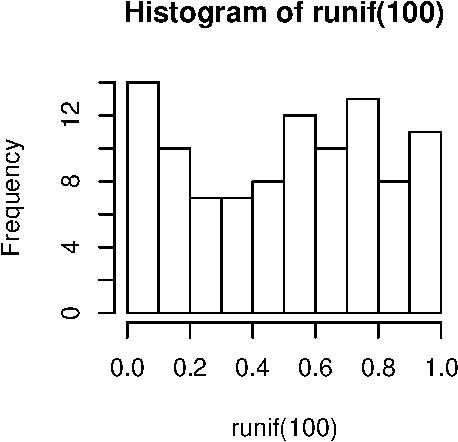
\includegraphics{main_files/figure-latex/random-1.pdf}
\caption{\label{pic1}Random picture}
\end{figure}

\hypertarget{references}{%
\section{References}\label{references}}

\end{document}
